\section*{Color Image Processing}

Light is made up of a spectrum of \textbf{electromagnetic radiation},
each wavelength having its own color.

The colors that humans and most animals perceive in an object are
determined by the nature of the light reflected from the object

For example, green objects reflect light with wave lengths primarily
in the range of 500 – 570 nm while absorbing most of the energy at
other wavelengths

Chromatic light spans the electromagnetic spectrum from approximately
400 to 700 nm

Human color vision is achieved through 6 to 7 million cones in each eye

\subsection*{Quality of a Chromatic Light Source}

\begin{itemize}
  \item \textbf{Radiance:} the total amount of energy that flows from
    the light source (measured in watts)
  \item \textbf{Luminance:} the amount of energy an observer
    perceives from the light source (measured in lumens)
  \item \textbf{Brightness:} a subjective (practically unmeasurable)
    notion that embodies the intensity of light
\end{itemize}

\subsection*{CIE Chromaticity Diagram}

\begin{itemize}
  \item Specifying colors systematically can be achieved using the
    CIE chromacity diagram
  \item On this diagram the \textbf{x-axis} represents the
    \textbf{proportion of red} and the \textbf{y-axis} represents the
    \textbf{proportion of green} used
  \item The proportion of blue used in a color is calculated as: $z
    = 1 – (x + y)$
\end{itemize}

\begin{figure}[H]
  \centering
  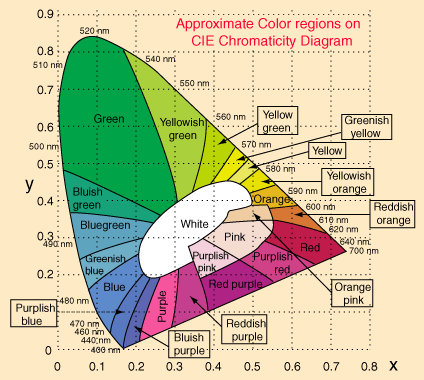
\includegraphics[width=0.8\linewidth]{images/cie_chromaticity_diagram.png}
  \caption{CIE Chromaticity Diagram Broken Down into Regions}
\end{figure}

\subsubsection*{Properties}

\begin{itemize}
  \item Any color located on the boundary of the chromacity chart is
    fully saturated
  \item The point of equal energy has equal amounts of each color
    and is the CIE standard for pure white
  \item Any straight line joining two points in the diagram defines
    all of the different colors that can be obtained by combining
    these two colors additively
  \item The above can be easily extended to three points
  \item This means the entire color range cannot be displayed based
    on any three colors
  \item The \textbf{triangle} shows the typical color gamut produced
    by RGB monitors
  \item The \textbf{strange shape} is the gamut achieved by high
    quality color printers
\end{itemize}

\begin{figure}
  \centering
  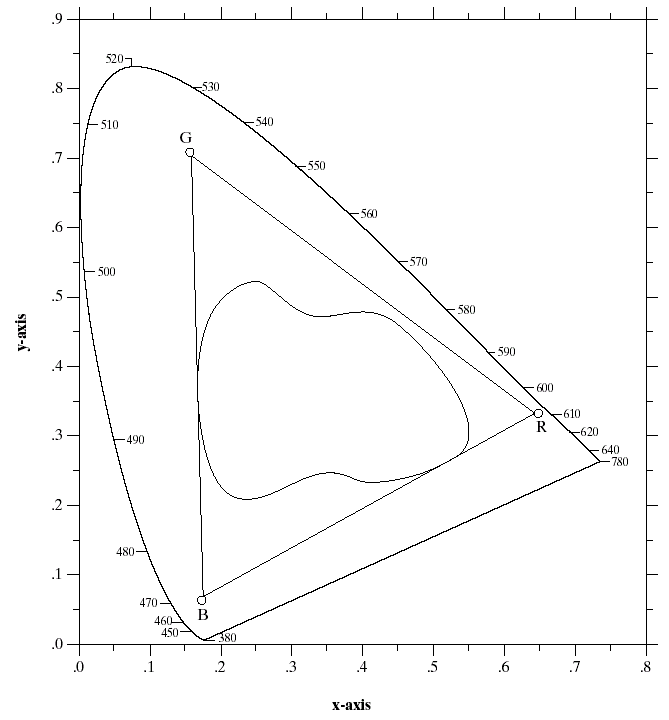
\includegraphics[width=0.8\linewidth]{images/cie_triangle.png}
  \caption{CIE Chromaticity Diagram with RGB Triangle and Printer Gamut}
\end{figure}

\subsection*{Color Models}

\subsubsection*{RGB Color Model}

\begin{itemize}
  \item Based on the Cartesian coordinate system
  \item Each color appears in its primary spectral components of
    \textcolor{MaterialRed900}{red},
    \textcolor{MaterialGreen900}{green}, and \textcolor{MaterialBlue900}{blue}

  \item RGB values are at 3 corners
  \item Cyan magenta and yellow are at \textbf{other three corners}
  \item Black is at the origin
  \item White is the corner \textbf{furthest from the origin}
  \item Different colors are points on or inside the cube represented
    by RGB vectors
\end{itemize}

\begin{minipage}{\linewidth}
  \begin{figure}[H]
    \centering
    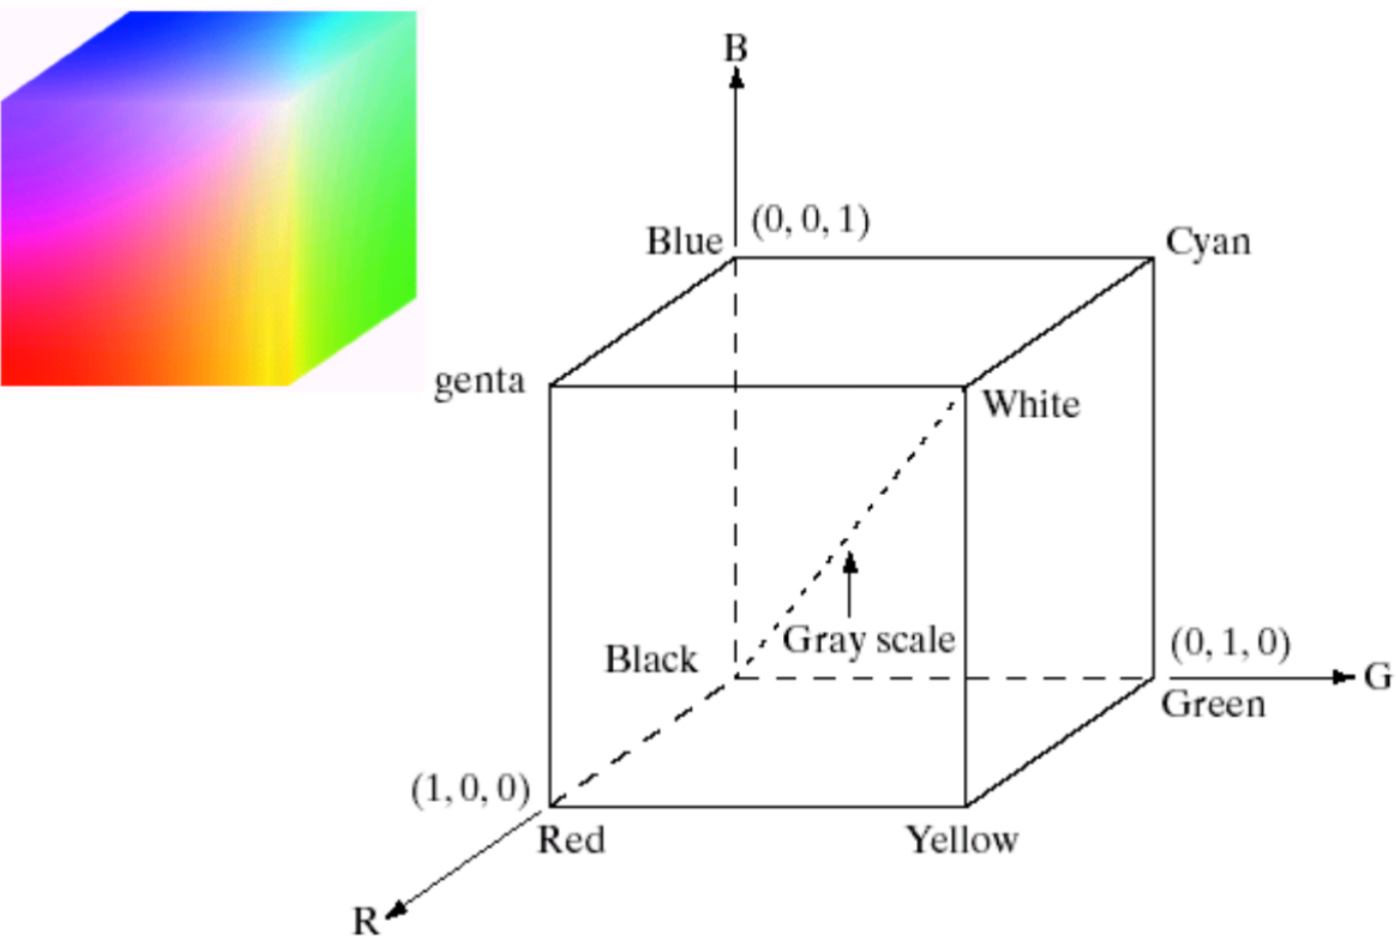
\includegraphics[width=\linewidth]{images/rgb_cube.png}
    \caption{RGB Color Cube}
  \end{figure}
\end{minipage}

\textbf{Properties:}

\begin{itemize}

  \item Images represented in the RGB color model consist of three
    component images – one for each primary color
  \item When fed into a monitor these images are combined to create a
    composite color image
  \item The number of bits used to represent each pixel is referred
    to as the \textbf{color depth}
  \item A 24-bit image is often referred to as a \textbf{full-color image} as
    it allows = 16,777,216 colors
\end{itemize}

\subsubsection*{HSI Color Model}

\textbf{Motivation:}

\begin{itemize}
  \item RGB is useful for hardware implementations related to the way
    in which the human visual system works, but \textbf{not very intuitive}
  \item People tend to use \textbf{hue, saturation and brightness}
  \item RGB is great for color generation, but HSI is great for color
    description
\end{itemize}

\textbf{Model Description:}

\begin{itemize}
  \item \textbf{Hue:} A color attribute that \textbf{describes a pure color}
    (pure yellow, orange or red)
  \item \textbf{Saturation:} Gives a measure of how much a pure
    color is \textbf{diluted with white light}
  \item \textbf{Intensity:} Brightness is nearly impossible to
    measure because it is so subjective. Instead we use intensity.
    Intensity is the same achromatic notion that we have seen in grey
    level images
\end{itemize}

If we \enquote{hold} the RGB cube at an angle such that we're staring
down the brightest point and the origin, we can see that the RGB cube
appears to be a hexagon.

The corners of the hexagon are the pure colors. White and black
coincide in this 2D view. Switching to 3D, the hexagon becomes a
hexagonal prism, with a white top and a black bottom.

\begin{figure}[H]
  \centering
  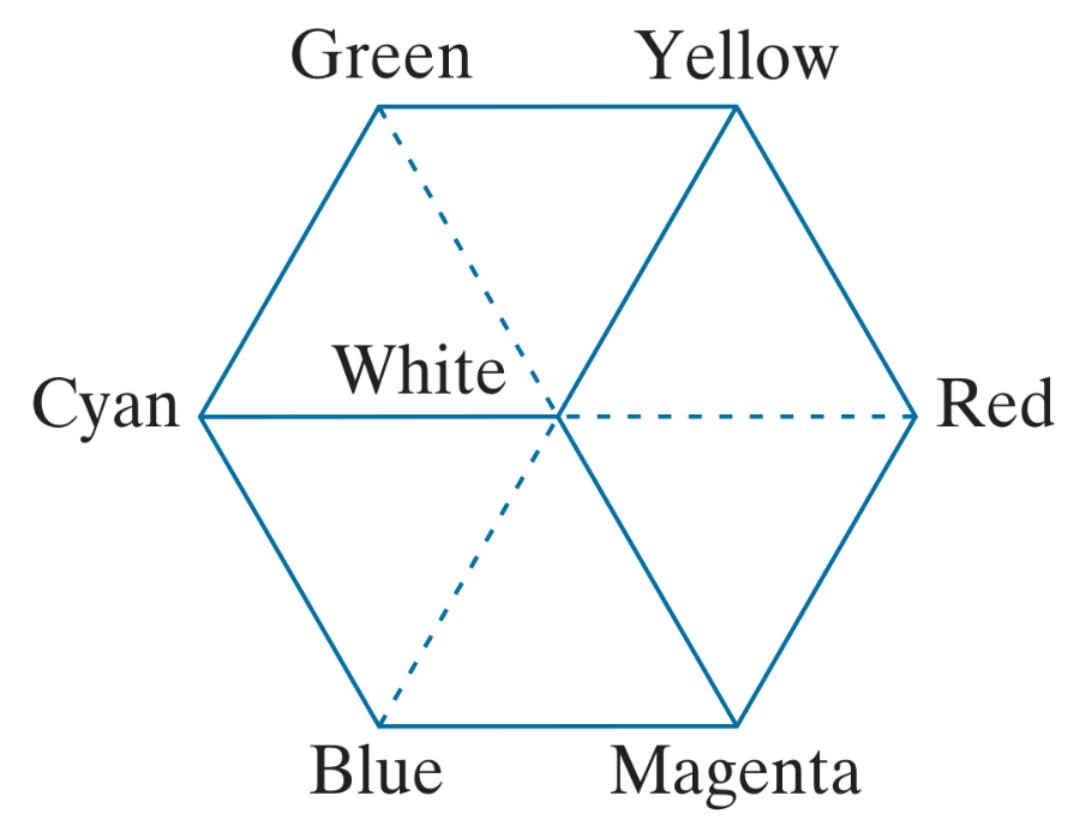
\includegraphics[width=0.6\linewidth]{images/hsi_hexagon.png}
  \caption{A \enquote{hexagon} obtained by looking at the RGB cube
  from a specific angle}
\end{figure}

\textbf{HSI}, unlike RGB, is based on the \textbf{cylindrical
coordinate system}. Intensity is a point on a line running from the
lowest point of the cylinder to the top. Hue and saturation are
angles around the cylinder.

Since the angles and the length are the only important things, the
HSI model can be visualized as the projection of a hexagon (hexagonal
prism), a circle (cylinder) or a triangle (triangular prism).

\begin{figure}[H]
  \centering
  \includegraphics[width=\linewidth]{images/hsi_projection.png}
  \caption{Different Projections of HSI}
\end{figure}

\subsubsection*{RGB to HSI Conversion}

\begin{fleqn}[1.5em]
  \begin{flalign*}
    & \theta \;=\;
    \cos^{-1}
    \Biggl(
      \frac{\tfrac{1}{2}\bigl[(R - G) + (R - B)\bigr]}
      {\sqrt{(R - G)^2 + (R - B)(G - B)}}
    \Biggr)\\[1.5em]
    & H \;=\;
    \begin{cases}
      \displaystyle \theta, & B \le G,\\[1ex]
      \displaystyle 360^\circ - \theta, & B > G.
    \end{cases}\\[1.5em]
    & S \;=\; 1 \;-\; \frac{3}{R + G + B}\,\bigl[\min(R,G,B)\bigr]\\[1.5em]
    & I \;=\; \tfrac{1}{3}\,(R + G + B)
  \end{flalign*}
\end{fleqn}

\subsubsection*{HSI to RGB Conversion}

\begin{itemize}
  \item \textbf{RG sector ($0\le H<120^\circ$)}
    \begin{fleqn}[1.5em]
      \begin{flalign*}
        & R = I\Bigl[1 + \frac{S\,\cos H}{\cos(60^\circ - H)}\Bigr]\\[1.5em]
        & G = 3I - \bigl(R + B\bigr)\\[1.5em]
        & B = I\,(1 - S)\\[1.5em]
      \end{flalign*}
    \end{fleqn}

  \item \textbf{GB sector ($120^\circ\le H<240^\circ$)}
    \begin{fleqn}[1.5em]
      \begin{flalign*}
        & R = I\,(1 - S)\\[1.5em]
        & G = I\Bigl[1 + \frac{S\,\cos\!\bigl(H -
        120^\circ\bigr)}{\cos\!\bigl(H - 60^\circ\bigr)}\Bigr]\\[1.5em]
        & B = 3I - \bigl(R + G\bigr)\\[1.5em]
      \end{flalign*}
    \end{fleqn}

  \item \textbf{BR sector ($240^\circ\le H\le 360^\circ$)}
    \begin{fleqn}[1.5em]
      \begin{flalign*}
        & R = 3I - \bigl(G + B\bigr)\\[1.5em]
        & G = I\,(1 - S)\\[1.5em]
        & B = I\Bigl[1 + \frac{S\,\cos\!\bigl(H -
        240^\circ\bigr)}{\cos\!\bigl(H - 180^\circ\bigr)}\Bigr]
      \end{flalign*}
    \end{fleqn}
\end{itemize}

\subsection*{Pseudocolor Image Processing}

\begin{itemize}
  \item Pseudocolor (also called \textit{false color}) image
    processing consists of assigning colors to grey values based on a
    specific criterion
  \item Mainly for human visualization
  \item Why? Humans can discern between \textbf{thousands of color
    shades} and intensities, compared to only about \textbf{two dozen
    or so} shades of grey
\end{itemize}

\begin{figure}[H]
  \centering
  \includegraphics[width=\linewidth]{images/pseudocolor.png}
  \caption{Example of a pseudocolor image. Source: NASA}
\end{figure}

\begin{itemize}
  \item \textbf{Goal:} Convert grayscale image to artificially colored image
  \item Intensity slicing $\rightarrow$ simplest, most common way
  \item Other types of transformations are more general; capable of a
    wider range of pseudocolor enhancement results
\end{itemize}

\subsubsection*{Intensity Slicing}

\begin{enumerate}
  \item First we consider an image as a 3D function mapping spatial
    coordinates to intensities (that we can consider \enquote{heights})
  \item Now consider placing planes at certain levels parallel to the
    coordinate plane
  \item If a value is one side of such a plane it is rendered in one
    color, and a different color if on the other side
\end{enumerate}

\begin{figure}[H]
  \centering
  \includegraphics[width=0.8\linewidth]{images/intensity_slicing.png}
  \caption{Geometric Interpretation of Intensity Slicing}
\end{figure}

\begin{algorithm}[ht]
  \SetAlgoLined
  \DontPrintSemicolon
  Let $[0,L-1]$ represent the grey scale\;
  Let $l_0$ represent black [$f(x,y)=0$] \;
  Let $l_{L-1}$ represent white [$f(x,y)=L-1$]\;
  Suppose $P$ planes perpendicular to the intensity axis are defined
  at levels $l_1,\,l_2,\,\dots,\,l_p$\;
  Assuming that $0 < P < L-1$ then the $P$ planes partition the grey
  scale into $P+1$ intervals $V_1,\,V_2,\,\dots,\,V_{P+1}$\;
  Grey level colour assignments can then be made according to the relation:
  \[
    f(x,y) \;=\; c_k
    \qquad\text{if}\;
    f(x,y)\,\in\,V_k
  \]
  where $c_k$ is the colour associated with the $k^\text{th}$
  intensity level $V_k$ defined by the partitioning planes at $l=k-1$
  and $l=k$\;
  \caption{Intensity Slicing}
\end{algorithm}
